% Adapted from the manuscript appendices; detailed attention moved from experiments.
\unnumberedchapter{Appendix}
\suppressfloats[t]
\label{ch:appendix}
\setcounter{section}{0}
\renewcommand{\thesection}{\Alph{section}}
\renewcommand{\thesubsection}{\thesection.\arabic{subsection}}
\counterwithin{figure}{section}
\counterwithin{table}{section}
\counterwithin{equation}{section}
\renewcommand{\theHsection}{appendix.\Alph{section}}
\renewcommand{\theHfigure}{appendix.\thesection.\arabic{figure}}
\renewcommand{\theHtable}{appendix.\thesection.\arabic{table}}
\renewcommand{\theHequation}{appendix.\thesection.\arabic{equation}}
\FloatBarrier
\section{Implementation Details and Additional Results}\label{app:additional}

The appendices provide implementation settings, numerical rules, supplementary prediction and case results, and descriptive attention maps.

Table~\ref{tab:shared-training-protocol} summarizes the settings shared by the Full model and ablation arms; their architectural differences are listed in Table~\ref{tab:ablation-arms}.

The exploratory station/window descriptors use eight clusters ($K=8$) and neither define event labels nor contribute a cluster-prediction loss.

\begin{table}[htbp]
\centering
\caption{Shared training, model, and task settings for the Full model and ablation arms.}
\label{tab:shared-training-protocol}
\footnotesize
\setlength{\tabcolsep}{6pt}
\renewcommand{\arraystretch}{1.05}
\begin{tabularx}{\linewidth}{@{}p{0.30\linewidth}Y@{}}
\toprule
Item & Setting \\
\midrule
Initialization and seed & Identical initial parameter values across arms; seed 42 \\
Optimizer and batch size & AdamW; batch size 16; weight decay 0.05 \\
Learning rate & $5\times10^{-5}$ initially; cosine decay to $10^{-6}$ \\
Sampling and training budget & Fourfold positive-window oversampling; at most 50 epochs per onset-limit run; early-stopping patience 40 \\
Curriculum & Onset limit~$\leq5\rightarrow$Onset limit~$\leq10\rightarrow$Onset limit~$\leq15$ \\
Checkpoint criterion & Validation station-identification F1 among candidates with report precision $\geq0.80$ and recall $\geq0.70$ \\
Threshold candidates & $\{0.45,0.50,0.55,0.60,0.65,0.70,0.75,0.80,0.85,0.88,0.90,0.94\}$ \\
Held-out evaluation & Freeze the selected checkpoint and threshold before evaluating the shared test episodes \\
Windowing and targets & 60-s windows; 30 historical and 30 future windows; seven workstation, four gantry, and four transport-robot targets \\
Event and matching rules & One-window internal gap filling; Onset limit~$\leq5/10/15$; three-window onset tolerance \\
Encoder and attention & Five blocks; hidden dimension 80; temporal/geographic/semantic heads $4/2/2$ \\
Graph and positional context & Geographic hop cutoff 4; five semantic neighbours; eight-dimensional Laplacian encoding \\
Pattern bank & 16 prototypes from length-three temporal patches \\
Far-onset enhancement & Onset-loss multiplier 2; positive weights $9/10/11$ for Onset limit~$\leq5/10/15$ \\
False-alarm weighting & Ordinary false-positive weight 2.5; additional hard-false-positive multiplier 2.2 \\
\bottomrule
\end{tabularx}
\end{table}

The joint training objective uses the following weights. Event occurrence, start, duration, and prefix losses have weights $2.4$, $2.0$, $2.0$, and $2.5$, respectively. The cold-history onset term has weight $2.2$ within the event-occurrence objective; focal modulation uses exponent $1.5$, and the internal differentiable F1 term has weight $0.8$. Future occupancy uses separate binary-cross-entropy, Dice, and IoU weights of $0.7$, $0.5$, and $0.35$. The reconstruction, supervised contrastive, cause, and turning-point/momentary losses have weights $0.2$, $0.05$, $0.1$, and $0.25$. Remaining-time regression has weight $0.5$ in stage~1 and $4.0$ during head-only stage~2.

The offline event CSV can retain a one-window event through score-event merging. PHGST-DM training instead constructs targets from the operational occupancy grid.

All state rules act on the original physical feature scale before input standardization. Let $q$, $B$, $S$, $U$, $I$, $R$, and $Z$ denote queue length, blocked seconds, starved seconds, unavailable fraction, inbound-wait seconds, route-delay seconds, and shortage propagation, respectively. At the 60-s resolution, a workstation has raw hot evidence if any of the following holds: (i) $q\geq2$ and $B+S>0$; (ii) $B\geq24$ and $q\geq1$; (iii) $B+S\geq24$ together with an upstream/downstream coupling ratio of at least $0.15$, $I\geq20$, $R\geq20$, $Z\geq0.25$, or $q\geq1$; (iv) $S\geq30$ and $Z\geq0.25$; (v) $S\geq18$ and either $I\geq20$ or $R\geq20$; or (vi) $B+S\geq24$ together with worker absence or labour saturation. An active workstation operating-variation flag combined with $U\geq0.5$ also supplies hot evidence. Worker absence uses unavailable fraction $\geq0.5$; labour saturation uses an activity cutoff of $0.8$ among present workers, with a presence tolerance of $0.05$. A gantry requires $B+S\geq18$ and either $I\geq20$ or $R\geq20$, whereas a transport robot requires $B+S\geq18$ and $I\geq20$; either handling type is also hot when $U\geq0.5$. When an operating-variation flag is active, evidence is retained only if $q\geq1$, $B+S\geq24$, or $U\geq0.5$. Raw indicators are filtered to remove runs shorter than eight one-minute windows, after which internal gaps of at most one window are filled. This retrospective occupancy grid supplies supervision; inference uses only the observed prefix.

For correspondence with the code, the disabled auxiliary-loss switches retain the implementation names \texttt{score}, \texttt{will}, \texttt{mark}, \texttt{time-to-start}, \texttt{STGNPP}, and \texttt{offline cluster-head}. These names identify inactive configuration options; the active occurrence loss $\mathcal{L}_{\mathrm{will}}$ remains part of the training objective. The offline cluster-head weight is zero, so the model is not trained to classify the offline clustering assignments.

The prefix-continuation cutoff is $1.5$ windows. Occupancy-run extraction for event union uses probability cutoff $0.45$, with both ongoing and upcoming union enabled; direct occupancy-state evaluation uses cutoff $0.55$. The configured gantry and transport-robot report thresholds are $0.72$ and $0.68$, respectively, alongside the validation-selected global operating point. Threshold selection first prefers candidates satisfying the validation precision requirement and then maximizes the configured station-identification F1; if none satisfies that requirement, it retains the highest-F1 validation candidate. The checkpoint precision/recall gates are applied separately. If no gated checkpoint is obtained throughout training, the retained ungated checkpoint with the best validation selection score is used. Neither fallback uses test predictions or test labels.

Evaluation counts refer to forecast-origin--resource pairs, so a persistent event may contribute at successive origins. Overlapping windows are not treated as independent observations for significance testing.

\FloatBarrier
\section{Supplementary prediction results}\label{app:supplementary-results}

\subsection{Temporal and resource-type results}

For Onset limit~$\leq15$, strict report recall is $0.574/0.522/0.433$ for onset distances within 5, 6--10, and beyond 10~min. Across the three limit-specific tasks, exact-onset accuracy among station-matched true positives is $0.896/0.844/0.831$, and onset-bucket accuracy is $0.921/0.918/0.920$. Workstation/gantry/robot F1 is $0.805/0.811/0.771$ at Onset limit~$\leq5$ and $0.751/0.840/0.639$ at Onset limit~$\leq15$. Aggregate event and timing results are in Table~\ref{tab:comparison-main}.

\subsection{Structural and pattern-modelling comparisons}

Beyond the main structural-ablation results, NoGroup has a strict report recall of $0.192$ for onsets beyond 10~min. Across limits, resource-type hmean is $0.505$--$0.536$ for Full, $0.360$--$0.384$ for NoGraph, and $0.365$--$0.396$ for NoCross. Figure~\ref{fig:key-device-entity} illustrates the corresponding trajectories: Full identifies both intervals about 5~min before NoInfo and WorkstationOnly, whose duration estimates remain at 6--8~min during the plotted 20-min reference plateau. NoCross reaches 14~min before declining to about 8~min.

\subsection{Stage-resolved sensitivity alignment}

Table~\ref{tab:oracle-pilot-ci} supplements Figure~\ref{fig:label-oracle-pilot} with point estimates and reported 95\% confidence intervals for the Ops labelling method. The results describe the 30-episode development pilot and should be interpreted as exploratory evidence.

\begin{table}[!htbp]

\centering
\caption{Production-sensitivity alignment of the Ops labelling method used by PHGST-DM in the development pilot.}
\label{tab:oracle-pilot-ci}
\footnotesize
\setlength{\tabcolsep}{8pt}

\renewcommand{\arraystretch}{1.1}
\begin{tabular*}{\linewidth}{@{\extracolsep{\fill}}lrr@{}}
\toprule
Metric & Point estimate & 95\% confidence interval \\

\midrule
NDCG@3 & 0.531 & [0.492, 0.570] \\
Positive Recall@2 & 55.556\% & [51.141, 59.971]\% \\
Positive Recall@3 & 68.519\% & [63.270, 73.768]\% \\
Weighted Recall@3 & 71.623\% & [66.052, 77.194]\% \\
Coverage@3$_{0.9}$ & 72.222\% & [66.974, 77.470]\% \\
\bottomrule
\end{tabular*}
\par\vspace{3pt}
\begin{minipage}{\linewidth}
\footnotesize
The pilot comprises 30 disturbance-free development episodes. These exploratory intervals do not establish superiority over the comparison methods or generalization to other disturbance conditions.
\end{minipage}
\end{table}



The mean weighted coverage of positive sensitivity by the top three candidates is $71.6\%$ under the pilot protocol. Early-, middle-, and late-stage NDCG@3 values are $0.421/0.339/0.770$, with the strongest alignment near order completion. 

\FloatBarrier
\section{Case selection and additional resource-level results}\label{app:case-details}

\subsection{Case selection and detailed trace observations}

The episode used for the main case study is \texttt{n10\_human1.0\_\_episode\_03}. The cutting workstation contributes 301 event-positive window--resource pairs. Devices with at least the median event count are first retained. Among them, the device with the most events in a single episode is selected, with ties resolved by PHGST-DM one-step F1. Its episode is then chosen based on the number and length of bottleneck segments. Figure~\ref{fig:key-device-baselines} reports the selected case. PHGST-DM estimates the short-event duration as 10--11~min; during the plotted 20-min reference plateau, estimates are 13--17~min, with state errors spanning 1--2 boundary windows. Plot truncation does not alter the 30-min prediction horizon.

\paragraph*{Mixed-condition probability map.}
Figure~\ref{fig:attn-prediction} uses a supplementary mixed-condition checkpoint and episode \texttt{n10\_mix\_all1.0\_\_episode\_03}, selected automatically for high bottleneck activity. It shows relative test windows $0$--$200$ across 20 rows: 15 target resources and five worker context nodes, omitting 18 buffers. The panels compare future labels, probabilities, and absolute errors. Probabilities are not thresholded reports, and this supplementary configuration does not represent the aggregate performance of the main \texttt{dense\_i1} model.

\begin{figure}[!htbp]
\centering
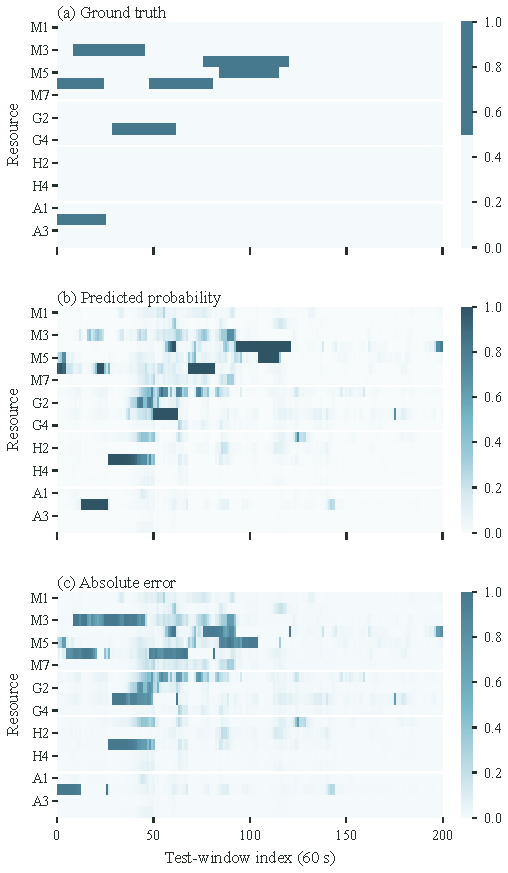
\includegraphics[width=\columnwidth,height=0.55\textheight,keepaspectratio]{figures/attention_heatmaps/fig08_prediction_heatmaps.pdf}
\caption{Future-event labels, predicted probabilities, and absolute errors for a mixed-condition episode (Onset limit~$\leq5$).}
\label{fig:attn-prediction}
\end{figure}

\paragraph*{Resource-level coverage.}

Table~\ref{tab:complete-6-1} provides per-resource counts and errors under the onset-qualified matching rule used in Table~\ref{tab:comparison-main}. Zero-support resources \texttt{robot\_2} and \texttt{robot\_3} are omitted. In this table, $n_{\mathrm{true}}$ and $n_{\mathrm{pred}}$ count reference and predicted event-positive forecast-origin--resource pairs, $P$ and $R$ denote precision and recall, and Dur MAE and Dur RMSE denote union duration errors in minutes. Device identifiers retain the simulator names so individual resources can be traced across data exports.

% Author confirms overall F1 = 80.4 percent and the same matching criterion as the main table.
% Per-device server exports are pending synchronization; do not infer replacement device counts from the aggregate score.
\begin{table}[!tbp]
\centering
\footnotesize
\setlength{\tabcolsep}{3pt}
\renewcommand{\arraystretch}{1.12}
\caption{Per-device event and duration performance at Onset limit~$\leq5$. Durations are in minutes. Zero-support resources (\texttt{robot\_2}, \texttt{robot\_3}) are omitted.}
\label{tab:complete-6-1}
\begin{tabularx}{\textwidth}{@{}lXXXXXXX@{}}
\toprule
Device & $n_{\mathrm{true}}$ & $n_{\mathrm{pred}}$ & $P$ & $R$ & F1-score & Dur MAE & Dur RMSE \\
\midrule
num00\_weld\_ws0 & 115 & 100 & 70.0\% & 60.9\% & 65.1\% & 5.31 & 7.11 \\
num00\_weld\_ws1 & 17 & 19 & 89.5\% & 100.0\% & 94.4\% & 1.54 & 2.76 \\
num01\_robotweld\_ws0 & 46 & 25 & 76.0\% & 41.3\% & 53.5\% & 6.04 & 7.56 \\
num02\_CNC$^\ast$\_ws0 & 301 & 343 & 76.7\% & 87.4\% & 81.7\% & 4.67 & 6.45 \\
num04\_groove\_ws0 & 20 & 27 & 55.6\% & 75.0\% & 63.8\% & 5.32 & 6.87 \\
num08\_bench\_ws0 & 186 & 162 & 91.4\% & 79.6\% & 85.1\% & 3.47 & 5.02 \\
num08\_bench\_ws1 & 94 & 101 & 93.1\% & 100.0\% & 96.4\% & 2.65 & 3.65 \\
gantry\_0 & 18 & 26 & 57.7\% & 83.3\% & 68.2\% & 3.35 & 4.85 \\
gantry\_1 & 31 & 34 & 76.5\% & 83.9\% & 80.0\% & 4.55 & 6.45 \\
gantry\_2 & 108 & 132 & 74.2\% & 90.7\% & 81.7\% & 3.59 & 5.56 \\
gantry\_3 & 121 & 127 & 81.1\% & 85.1\% & 83.1\% & 3.56 & 5.04 \\
robot\_0 & 15 & 10 & 90.0\% & 60.0\% & 72.0\% & 4.01 & 6.14 \\
robot\_1 & 30 & 28 & 82.1\% & 76.7\% & 79.3\% & 5.03 & 6.80 \\
\bottomrule
\end{tabularx}
\end{table}


\FloatBarrier
\section{Supplementary attention analysis}\label{app:attention-analysis}

\subsection{Historical attention and onset-limit comparisons}
Figure~\ref{fig:attn-temporal} compares historical attention under normal and upcoming bottleneck conditions using the protocol in Section~\ref{sec:attention-protocol}. Both maps contain prominent bands around history steps 12--15 and 25--30, indicating that the model draws on multiple historical regions. The upcoming-minus-normal map shows localized increases and decreases around these bands. This pattern is consistent with selective use of historical operating context when forecasting an emerging bottleneck.

\begin{figure}[hbp]
\centering
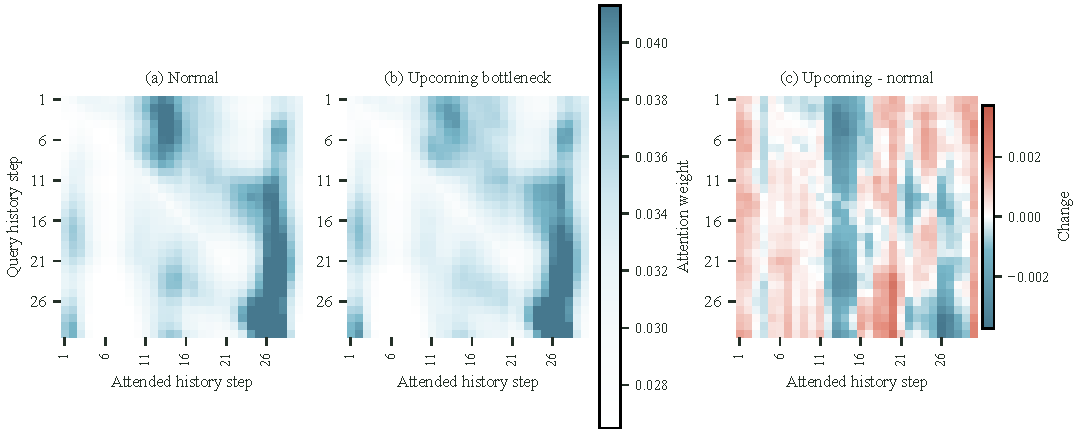
\includegraphics[width=0.98\textwidth,height=0.66\textheight,keepaspectratio]{figures/attention_heatmaps/fig04_temporal_attention_states.pdf}
\caption{Temporal attention over 30 history windows: (a)~normal; (b)~upcoming; (c)~upcoming-minus-normal.}
\label{fig:attn-temporal}
\end{figure}

\begin{figure}[!tbp]
\centering
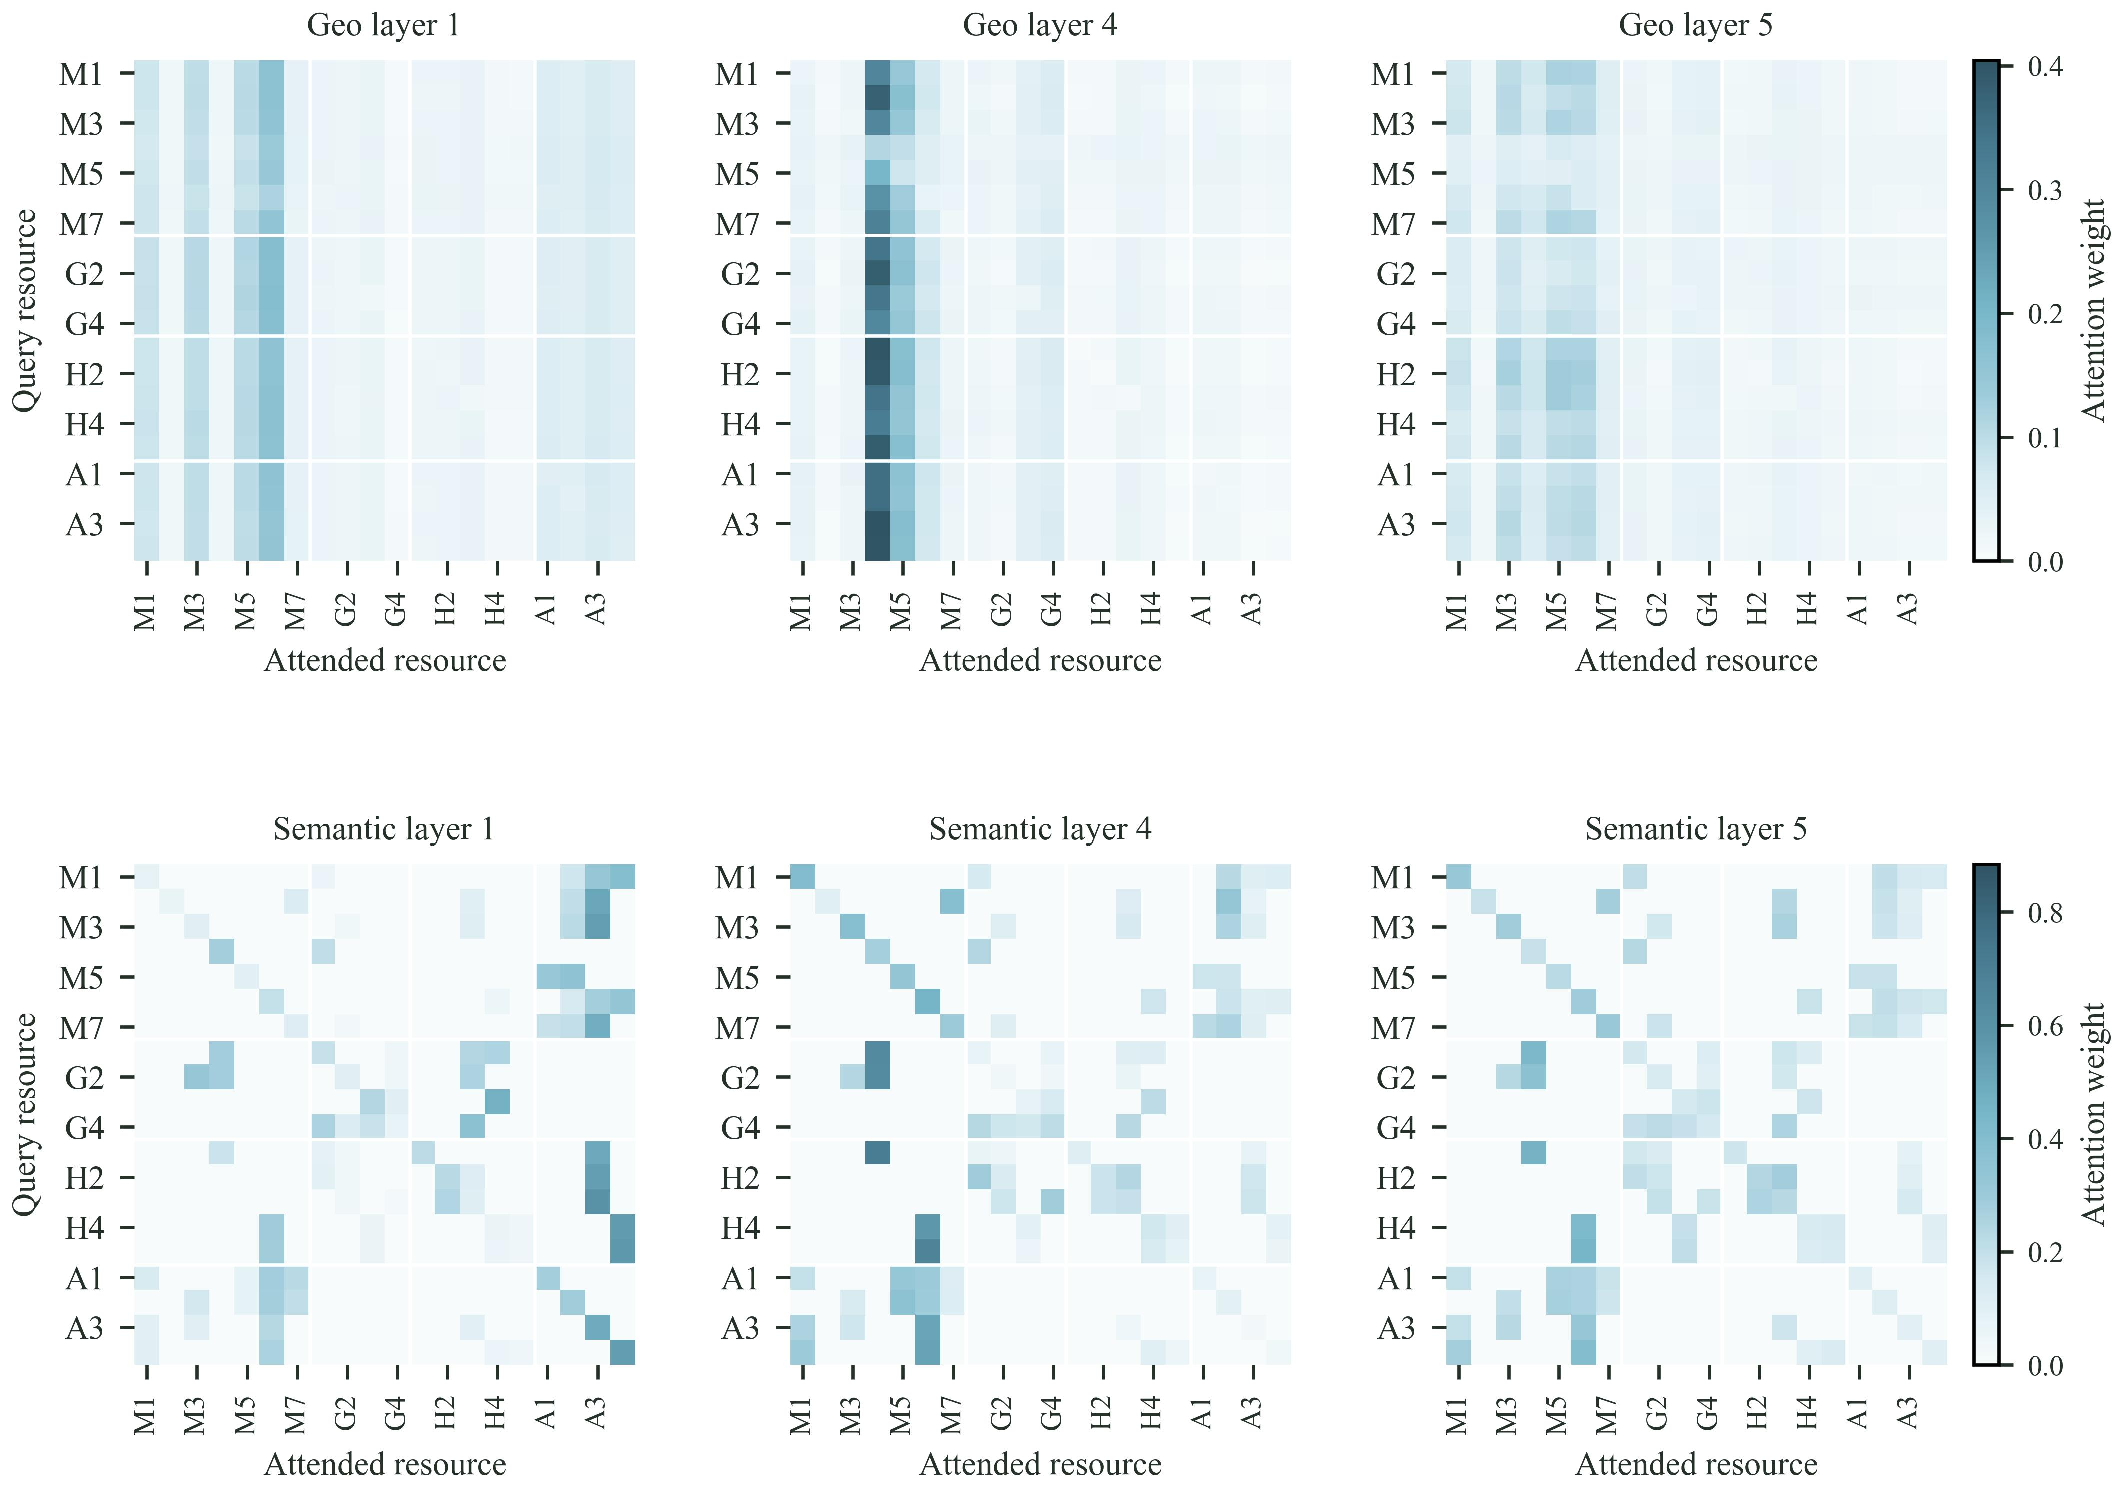
\includegraphics[width=0.92\textwidth,height=0.66\textheight,keepaspectratio]{figures/attention_heatmaps/fig05_layerwise_upcoming_attention_selected.pdf}
\caption{Geographic (upper) and semantic (lower) attention in selected encoder layers 1, 4, and 5.}
\label{fig:attn-layers}
\end{figure}

Figure~\ref{fig:attn-layers} reveals complementary changes across encoder layers. Geographic attention is distributed across several workstation columns in layer~1, becomes concentrated around M3 in layer~4, and is more distributed again in layer~5. Semantic attention remains sparse and resource-specific, with prominent links involving workstations, workers, and AGVs. Together, these views show that resource information is reweighted across layers and combined through distinct geographic and semantic patterns. Appendix~\ref{app:layerwise-attention} presents all five layers.

Figure~\ref{fig:attn-horizons} compares upcoming-minus-normal resource attention under Onset limit~$\leq5/10/15$, using 96 samples per condition. Geographic maps retain a common emphasis on the M3--M5 workstation region, while the magnitudes and extent of the changes vary across onset limits. Semantic maps show localized positive and negative changes, including recurring links to M3--M4 across resource types. Thus, the models share recurring resource associations while adjusting the allocation of attention to the admissible onset range.

\begin{figure}[!tbp]
\centering
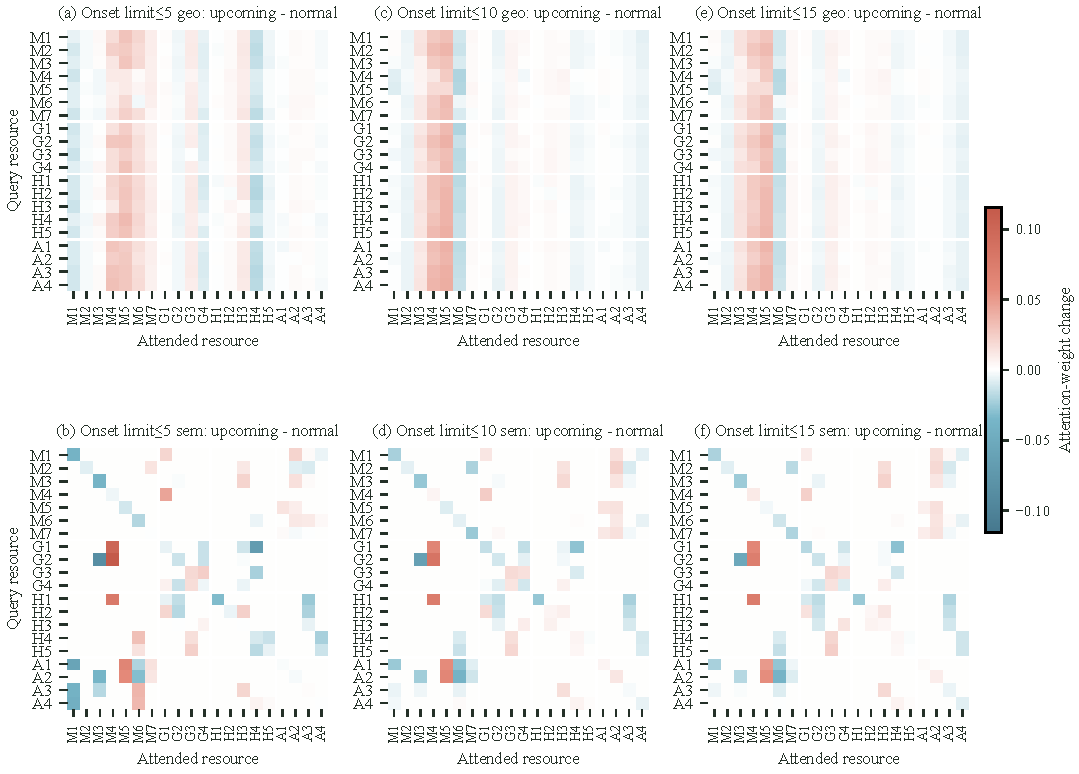
\includegraphics[width=0.98\textwidth,height=0.66\textheight,keepaspectratio]{figures/attention_heatmaps/fig07_horizon_attention_change.pdf}
\caption{Upcoming-minus-normal attention change across onset limits 5/10/15 (upper: geographic; lower: semantic).}
\label{fig:attn-horizons}
\end{figure}

\paragraph*{Learned cross-resource allocation under mixed operating conditions.}
Attention sampling and averaging follow the protocol in Section~\ref{sec:attention-protocol}. Figure~\ref{fig:attn-change} presents the resource-level change maps underlying the type-level summary in the main text.

Average attention under upcoming and ongoing conditions is compared with that under normal conditions. Colour indicates increased or decreased weight; the absolute reference matrices are retained below.

\begin{figure}[!htbp]
\centering
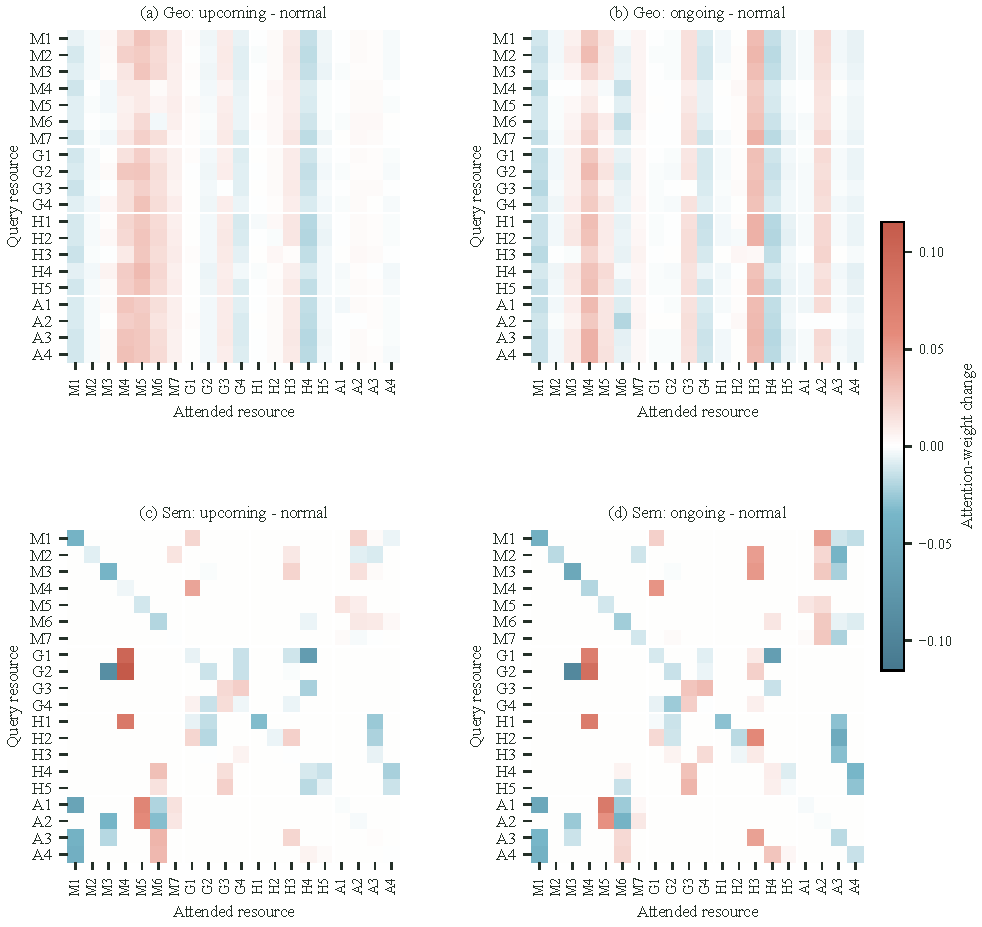
\includegraphics[width=0.92\textwidth,height=0.66\textheight,keepaspectratio]{figures/attention_heatmaps/fig03_resource_attention_change.pdf}
\caption{Redistribution of resource attention under upcoming and ongoing conditions relative to normal conditions (coral: increase; blue: decrease).}
\label{fig:attn-change}
\end{figure}



\subsection{Complete resource and layer matrices}
\label{app:absolute-attention}
\label{app:layerwise-attention}
Figures~\ref{fig:attn-states} and~\ref{fig:attn-layers-all} retain the absolute resource averages and all five layers corresponding to the selected views in this appendix. Layer-wise matrices share the same scale within each branch. Attention weights describe learned associations, not causal effects or layer-wise accuracy contributions.

\begin{figure}[!tbp]
\centering
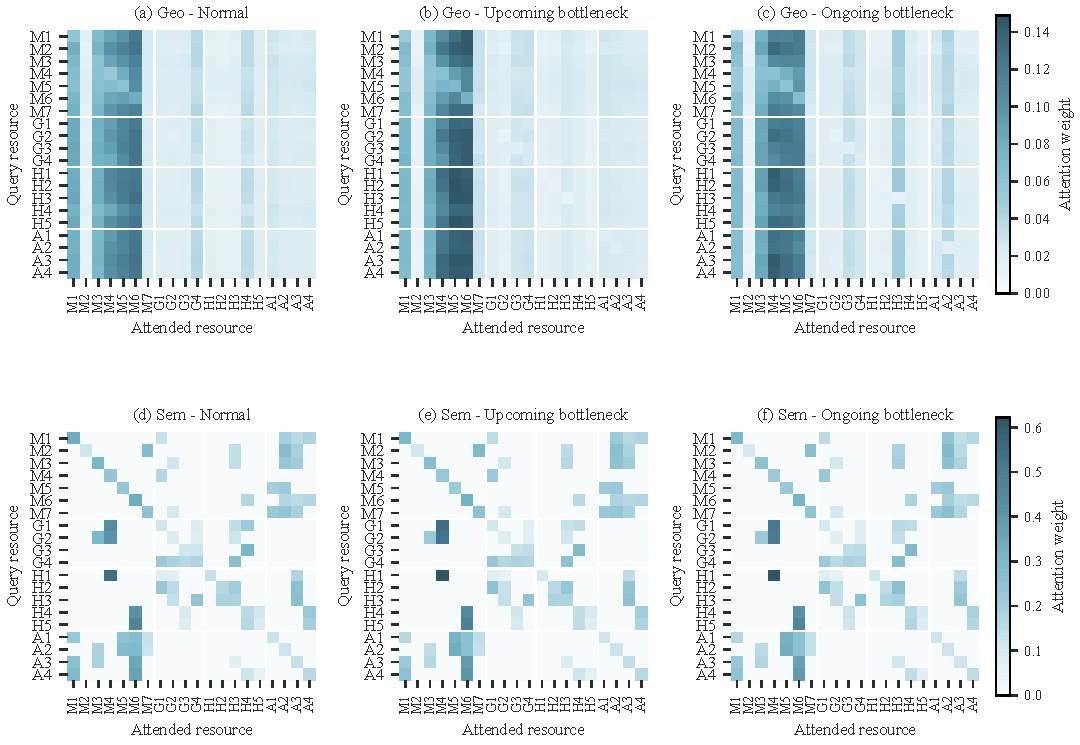
\includegraphics[width=0.92\textwidth,height=0.66\textheight,keepaspectratio]{figures/attention_heatmaps/fig02_resource_attention_states.pdf}
\caption{Absolute geographic (upper) and semantic (lower) resource attention under normal, upcoming, and ongoing conditions.}
\label{fig:attn-states}
\end{figure}

\begin{figure}[!tbp]
\centering
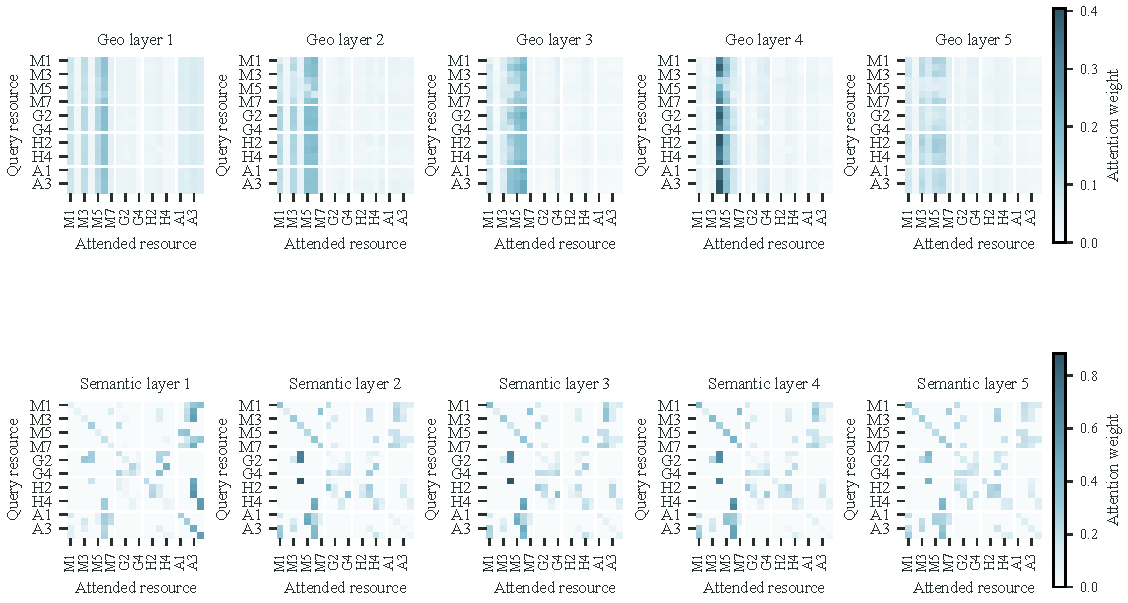
\includegraphics[width=0.94\textwidth,height=0.66\textheight,keepaspectratio]{figures/attention_heatmaps/fig05_layerwise_upcoming_attention.pdf}
\caption{Geographic (upper) and semantic (lower) attention across encoder layers 1--5 for upcoming samples.}
\label{fig:attn-layers-all}
\end{figure}

